Рассмотрим описанные алгоритмы поиска ключей в словаре. Пусть производится поиск ключа $key$ в словаре $a$ длиной $len$.

\section{Поиск полным перебором}
Алгоритм проходит от 1-го элемента до len-го в поиске полного совпадения ключа. В случае, если ключ был найден, производится досрочный выход из поиска записи. Если после прохода по всем элементам словаря совпадение не было обнаружено, сообщается о том, что ключ не был найден.

Схема алгоритма приведена на рисунке 2.1
\begin{figure}[h]
	\begin{center}
		{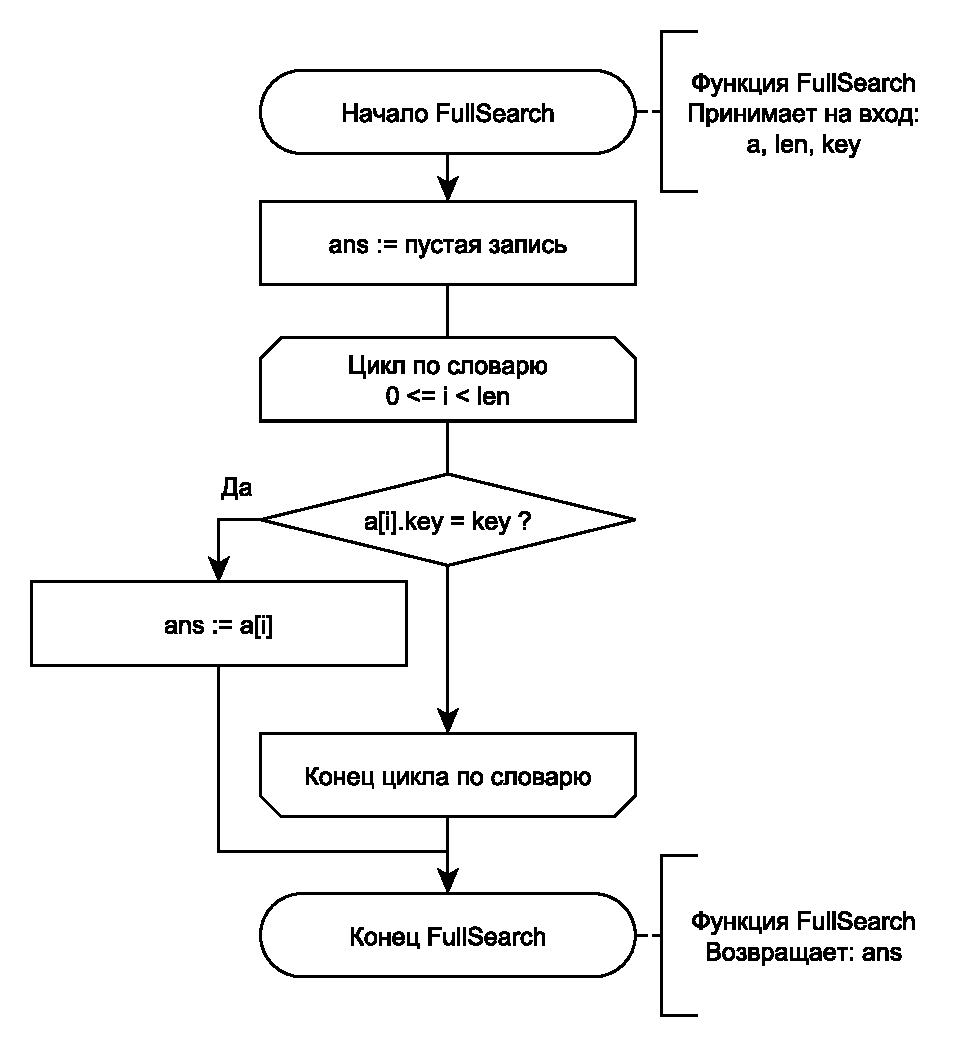
\includegraphics[height=20cm, width = 14cm]{FullSearch}}
		\caption{Поиск полным перебором}
	\end{center}
\end{figure}

\section{Поиск половинным разбиением}
Данный метод может применяться только для упорядоченного массива. Описание работы приведено для случая, когда алгоритм повторяет операцию поиска для интервала индексов массива, изначально содержащим все индексы от 0 до $len-1$. Эти два значения называются левой (l) и правой (r) границей массива соответственно. Алгоритм выбирает элемент с индексом $mid = round((l+r)/2)$ и сравнивает его ключ с искомым. В случае, если искомый ключ больше ключа mid, левая граница ставится на mid+1, если меньше, то праваой границе присваивается mid-1. Если произошло совпадение, то ключ найден и происходит выход из функции. Если правая граница оказалась меньше левой, то это говорит о том, что искомого ключа в словаре нет.

Схема алгоритма приведена на рисунке 2.2
\begin{figure}[h]
	\begin{center}
		{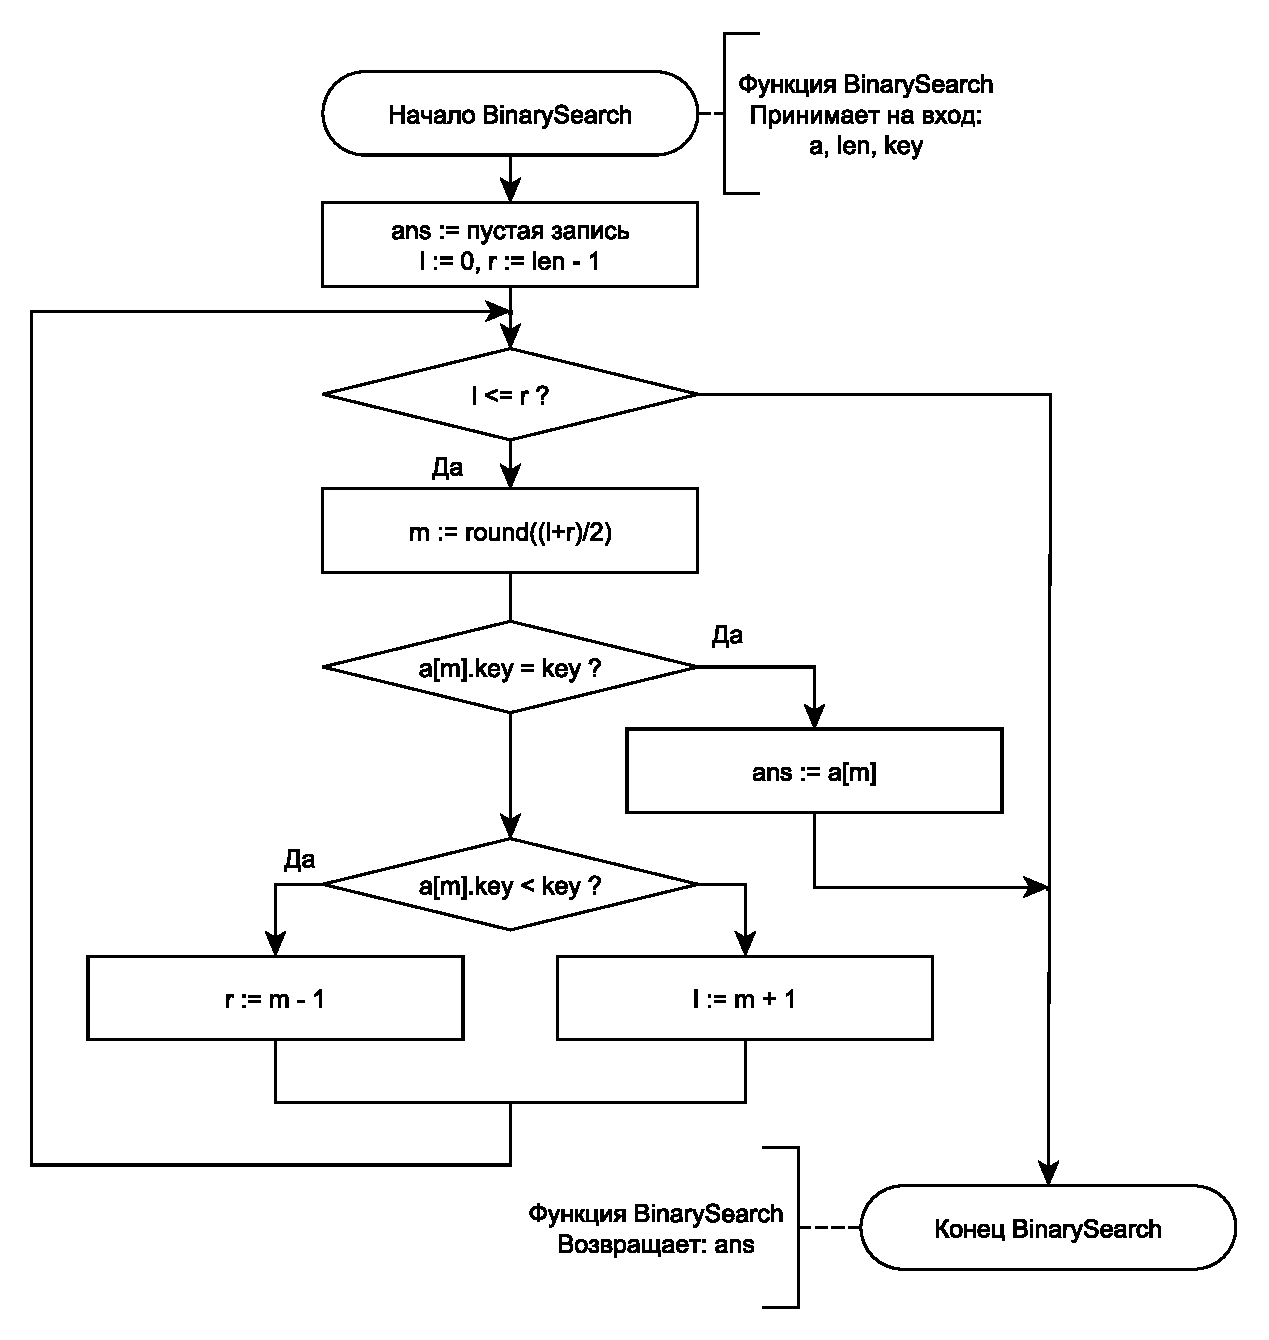
\includegraphics[height=20cm, width = 14cm]{BinarySearch}}
		\caption{Поиск половинным разбиением}
	\end{center}
\end{figure}

\section{Поиск с сегментами}
Для использования данного поиска требуется предварительно провести сегментацию словаря (схема алгоритма приведена на рисунке 2.3.). В данной работе сегментация производится по последней цифре номера карты, так как в этом случае элементы словаря будут равномерно распределены между сегментами.

Структура сегмента состоит из двух полей:
\begin{enumerate}
	\item ключ - последняя цифра для всех ключей словаря;
	\item массив пар - словарь из значений соответсвующих ключу.
\end{enumerate}

\begin{figure}[h]
	\begin{center}
		{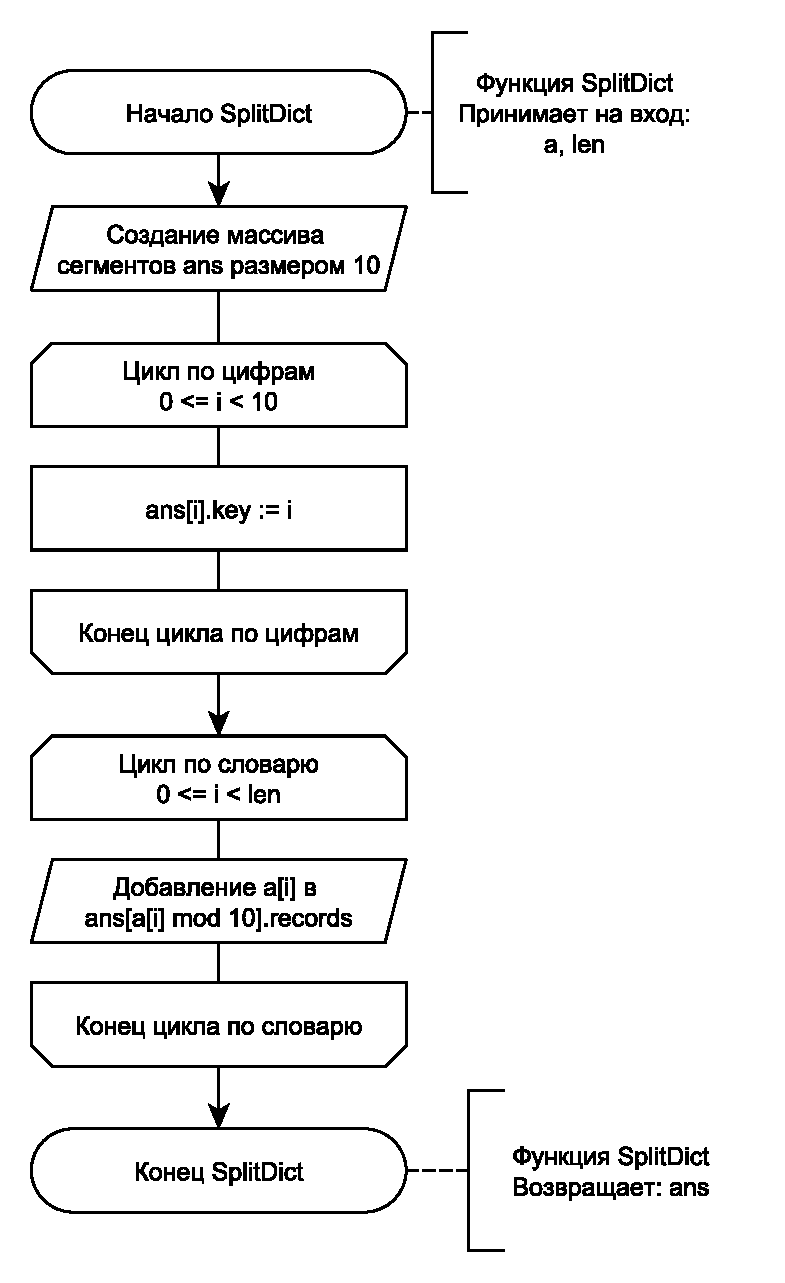
\includegraphics[height=20cm, width = 14cm]{Segmentation}}
		\caption{Разбиения словаря по сегментам}
	\end{center}
\end{figure}

Алгоритм использует вышеописанный полный поиск сначала для нахождения нужного сегмента, а после ищет нужный ключ среди элементов сегмента.

Схема алгоритма приведена на рисунке 2.4
\begin{figure}[h]
	\begin{center}
		{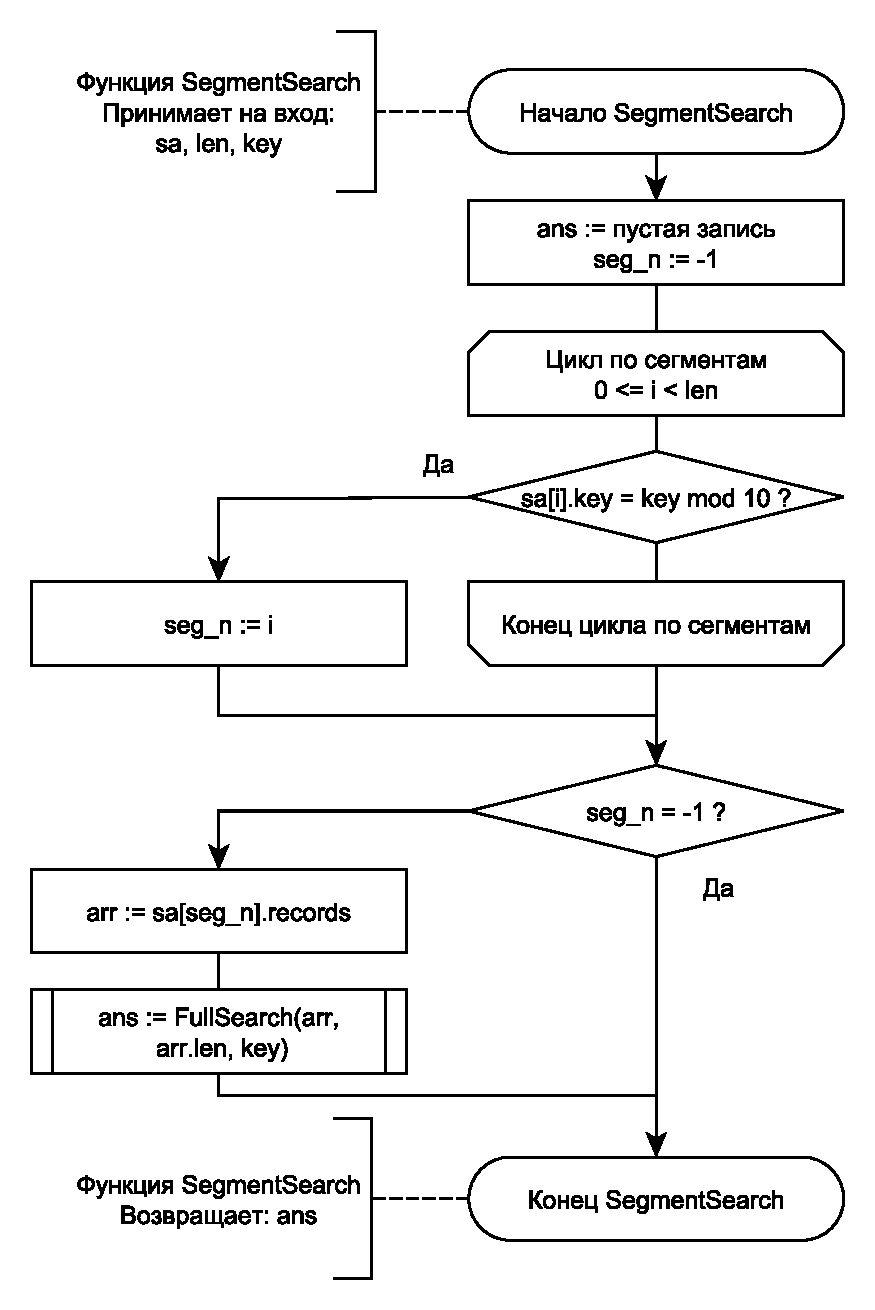
\includegraphics[height=20cm, width = 14cm]{SegSearch}}
		\caption{Поиск с сегментами}
	\end{center}
\end{figure}


\section{Требования к программному обеспечению}
Для полноценной проверки и оценки алгоритмов необходимо выполнить следующее.
\begin{enumerate}
	\item Предоставить возможность ввода искомого ключа и проверяемого алгоритма.
	\item Реализовать функцию замера процессорного времени, затраченного функциями и подсчёта статистических данных.
\end{enumerate}


\section{Заготовки тестов}
При проверке алгоритма необходимо будет использовать следующие классы тестов:
\begin{itemize}
	\item поиск отсутствующего номера карты;
	\item поиск первого и последнего номера в словаре.
\end{itemize}

\section*{Вывод}
Результатом конструторской части стало схематическое описание алгоритмов поиска, сформулированны тесты и требования к программному обеспечению.


